\chapter{Versuch 1 - Bestimmung der Tonhöhe eines akustischen Signals}
\label{chap:VERSUCH_1}


\section{Fragestellung, Aufbau, Messmittel}
\label{chap:VERSUCH_1_FRAGESTELLUNG}

\subsection*{Fragestellung}


\subsection*{Aufbau}



\subsection*{Messmittel}
\begin{itemize}
	\item Mikrophon
	\item Klarinette
\end{itemize}

\section{Messwerte}
\label{chap:VERSUCH_1_MESSWERTE}



Zwei Schwinungen, aus den späteren abschnitten (die ersten 50.000 Werte wurden übersprungen, weil das Signal zu verworren war)
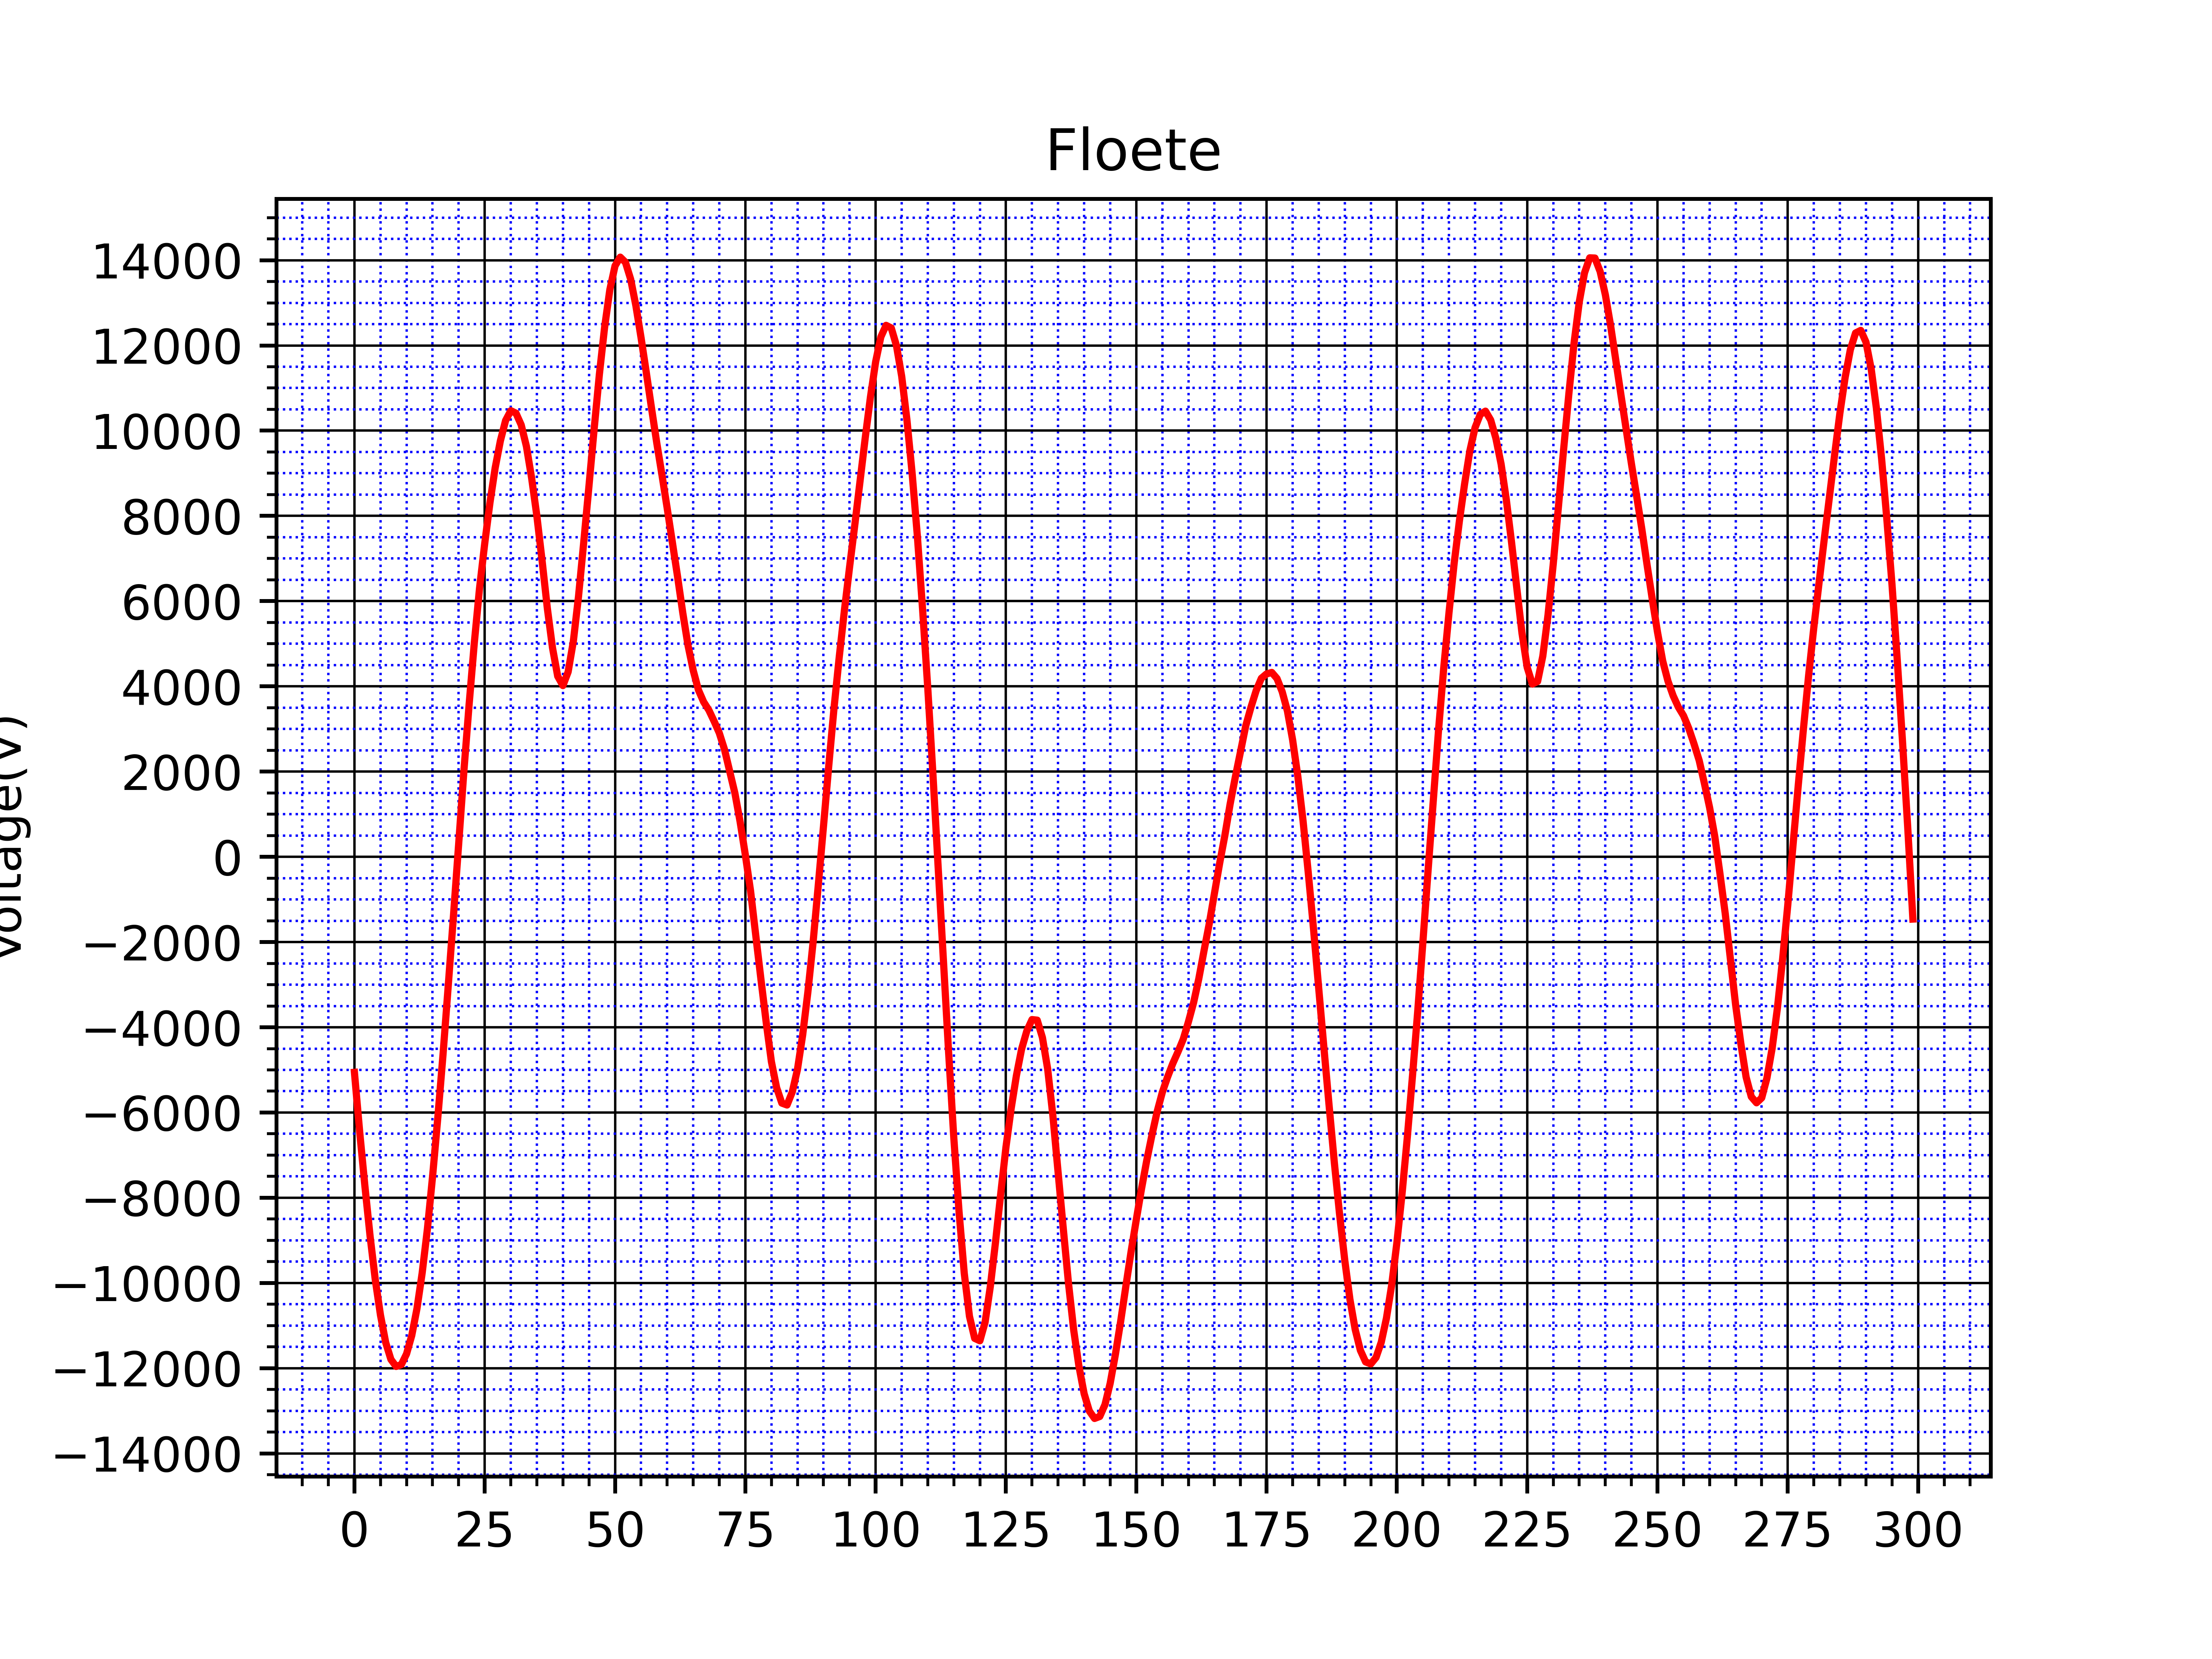
\includegraphics[scale=0.75]{media/Signal_Raster}

\section{Auswertung}
\label{chap:VERSUCH_1_AUSWERTUNG}



\section{Interpretation}
\label{chap:VERSUCH_1_INTERPRETATION}